\chapter{Related Works}
\label{cha:relatedworks}

\section{Huang's Model}


The work of \cite{HuangSocherEtAl2012} is based on the model of \cite{CollobertWeston2008}. They try to make embedding vectors with richer semantic information. They had two major innovations to accomplish this goal : The first innovation is using global information from the whole text to assist local information, the second innovation is using the multiple word vectors to represent polysemy. 

Huang thinks \cite{CollobertWeston2008} use only "local context". In the process of training vectors, they used only 10 words as the context for each word, counting the center word itself, there are totally 11 words' information. 
This local information can not fully exploit the semantic information of the center word. Huang used their neural network directly to compute a score as the "local score". 

And then Huang proposed a "global information", which is somewhat similar to the traditional bag of words model. Bag of words is about accumulating One-hot Representation from all the words of the article together to form a vector (like all the words thrown in a bag), which is used to represent the article. Huang's global information used the average weighted vectors from all words in the article (weight is word's idf), which is considered the semantic of the article. 
He connected such semantic vector of the article (global information) 
with the current word's vector (local information) to form a new vector with double size as an input, and then used the C$\&$W's network to calculate the score. Figure [huang] shows such structure.
With the "local score" from original C$\&$W approach and "Global score" from improving method based on the C$\&$W approach, Huang directly add two scores as the final score. The final score would be optimized by the pair-wise target function from C$\&$W. Huang found his model can capture better semantic information. \\

\begin{figure}[!ht]
  \centering
	\fbox{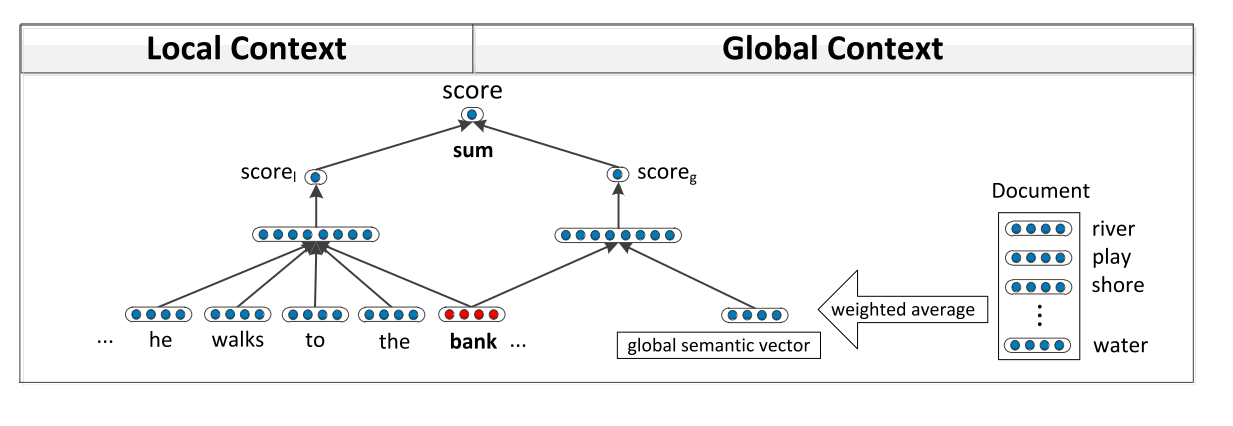
\includegraphics[width=0.9\textwidth]{huang} }
	\caption{The network structure from \citep{HuangSocherEtAl2012}}
	\label{fig:huang}
\end{figure}


The second contribution of this paper is to represent polysemy using multiple embeddings for a single word. For each center word, he took 10 nearest context words and calculated the weighted average of the embeddings of these 10 word vectors (idf weights) as the context vector. Huang used all context vectors to do a k-means clustering. He relabel  each word  based on the clustering results (different classes of the same words would be considered as different words to process). Finally he re-trained the word vectors. Table~\ref{tab:huang} gives some examples from his model's results.\\


\begin{table}[tb]
\begin{center}
\caption{Senses computed with Huang's network and their nearest neighbors.} 
\label{tab:huang}
\vspace{2mm}
 \begin{tabular}{|l|l|}
  \hline
  Center Word &Nearest Neighbors \\
  \hline  
  bank$\_$1 & corporation, insurance, company\\
  \hline
  bank$\_$2 & shore, coast, direction\\
  \hline
  star$\_$1 & movie, film, radio\\
  \hline
  star$\_$2 & galaxy, planet, moon\\
  \hline
  cell$\_$1 & telephone, smart, phone\\
  \hline
  cell$\_$2 & pathology, molecular, physiology\\
  \hline
  left$\_$1 & close, leave, live\\
  \hline
  left$\_$2 & top, round, right\\
  \hline
 \end{tabular}
\end{center}
\end{table}

\section{EM-Algorithm based method}


\cite{TianDaiEtAl2014} proposed an approach based on the EM-algorithm from . This method is the extension of the normal skip-gram model. They still use each center word to predict several context words. The difference is that each center word can have several senses with different probabilities. The probability should represent the relative frequency of the sense in the corpus. For example, considering $bank_1$ in the sense of "side of the river" and $bank_2$ meaning "financial institution". Usually $bank_1$ will have a smaller probability and $bank_2$. We can say in the corpus, in most sentences of the corpus the word "bank" means "financial institution" and in other fewer cases it means "side of the river". 

\paragraph{Objective Function}\

Considering $w_I$ as the input word and $w_O$ as the output word, $(w_I,w_O)$ is a data sample. The input word $w_I$ have $N_{w_I}$ prototypes, and it appears in its $h_{w_I}$-th prototype, i.e., $h_{w_I}\in \{1,..,N_{w_I}\}$ [] The prediction $P(w_O|w_I)$ is like the following formula
$$p(w_O|w_I)=\sum^{N_{w_I}}_{i=1}P(w_O|h_{w_I}=i,w_I)P(h_{w_I}=i|w_I)=\sum^{N_{w_I}}_{i=1}\frac{exp(U^{\mathrm{T}}_{w_O}V_{w_I,i})}{\sum_{w\in W exp(U^\mathrm{T}_w V_{w_I,i})}}P(h_{w_I}=i|w_I)$$
where $V_{w_I,i}\in R^d$ refers to the d-dimensional "input" embedding vector of $w_I$'s $i$-th prototype and $U_{w_O}\in R^d$ represents the "output" embedding vectors of $w_O$. Specifically, they use the Hierarchical Softmax Tree function to approximate the probability calculation. 

\begin{table}[tb]
	\begin{center}
		\caption{Word senses computed by \citeauthor{TianDaiEtAl2014}}
		\label{tab:tian}
		\vspace{2mm}
		\begin{tabular}{|l|l|l|}
			\hline
			word & Prior Probability & Most Similar Words \\
			\hline  
			apple$\_$1 & 0.82 & strawberry, cherry, blueberry\\
			\hline
			apple$\_$2 & 0.17 & iphone, macintosh, microsoft\\
			\hline
			bank$\_$1 & 0.15 & river, canal, waterway\\
			\hline
			bank$\_$2 & 0.6 & citibank , jpmorgan, bancorp\\
			\hline
			bank$\_$3 & 0.25 & stock, exchange, banking\\
			\hline
			cell$\_$1 & 0.09 & phones cellphones, mobile\\
			\hline
			cell$\_$2 & 0.81 & protein, tissues, lysis\\
			\hline
			cell$\_$3 & 0.01 &locked , escape , handcuffed\\
			\hline
		\end{tabular}
	\end{center}
	
\end{table}

\paragraph{Algorithm Description}\ 

Particularly for the input word $w$, they put all samples ($w$ as the input word) together like $\{(w, w_1), (w, w_2), (w, w_3) ... (w, w_n)\}$ as a group. Each group is based on the input word. So the whole training set can be separated as several groups. For the group mentioned above, one can assume the input word $w$ has $m$ vectors ($m$ senses), each with the probability $p_j (1 \leq j \leq m)$. And each output word $w_i (1 \leq i\leq n)$ has only one vector. 

 In the training process, for each iteration, they fetch only part of the whole training set and then split it into several groups based on the input word. In each E-step, for the group mentioned above, they used soft label $y_{i,j}$ to represent the probability of input word in sample $(w,w_i)$ assigned to the $j$-th sense. The calculating of $y_{i,j}$ is based on the value of sense probability and sense vectors. After calculating each $y_{i,j}$ in each data group, in the M-step, they use $y_{i,j}$ to update sense probabilities and sense vectors from input word, and the word vectors from output word. Table~\ref{tab:tian} lists some results from this model.

\section{A Method to Determine the Number of Senses}
\cite{neelakantan2015efficient} comes up with two different models, the first one is the MSSG (Multi-Sense Skip-gram) model, in which the number of senses for each word is fixed and decided manually. The second one is NP-MSSG  (Non-Parametric MSSG) which is based on the MSSG model , the number of senses for each word in this model is not fixed and can be decided dynamically by the model itself.


\paragraph{MSSG}\

\gls{C} is the given corpus containing the sentences/documents of words. \gls{N} is the number of different words in the corpus \gls{C}. \gls{D} is the vocabulary (the set of \gls{N} different words in the corpus \gls{C}). Considering a word $w_t$ in some sentence $S = (w_1,w_2,\ldots,w_{T-1},w_{T})$ from corpus \gls{C}, where $t$ is some position of $S$ and $T$ is the length of $S$, define $Context(w) = (w_{,\max(t-c,1)},\ldots,w_{t-1},w_{t+1},\ldots,w_{,\min(t+c,T)})$, and $c$ is the number of words before and after $w_t$ in the $Context(w)$. 

In the MSSG model, each word has $S$ senses ($S$ is set advance manually. Like huang's model, MSSG model uses the clustering, but its clustering strategy is different. Assuming each word has a context vector, which is summed up by all word vectors in the context. Huang's model do clustering on all context vectors (calculated by the weighted average of word vectors) from the corpus. While for MSSG model, they do clustering based on each word, that is each word has its own context clusters. Another thing is that MSSG only records the information (vector) of context cluster center for each word. For example, word $w$ has $S$ clusters , it has only $S$ context vectors. And in the initialization, these $S$ context vectors are set randomly. When there is a new context of word $w$, the model will firstly check which cluster this context should belong to and then use this new context vector to update the vector of selected context cluster center. 

Specifically, each word has a global vector, $S$ sense vectors and $S$ context cluster center vectors. All of them are initialized randomly. For word $w_t$, its global vector is $v_g(w_t)$ and its context vectors are $v_g(w_{t-c}),\ldots,v_g(w_{t-1}),v_g(w_{t+1}),\ldots,v_g(w_{t+c})$. $v_{context}(c_t)$ is the average context vector calculated by the average of these $2c$ global word vectors. And $w_t$'s sense vectors are $v_s(w_t,s) (s=1,2,\ldots,S)$ and the context cluster center vectors are $\mu(w_t,s) (s=1,2,\ldots,S)$. The architecture of the MSSG is like Figure \ref{fig:MSSG} when $c=2$. It uses the following formula to select the best cluster center:
$$s_t=\arg\max_{s=1,2,\ldots,S} sim(\mu(w_t,s),v_{context}(c_t)) $$
where $s_t$ is index of selected cluster center and $sim$ is the cosine similarity function. The selected context cluster center vector $\mu(w_t,s_t)$ will be updated with current context vector $v_{context}(c_t)$. And then the model selects $v_(w,s_t)$ as current word's sense. The rest thing is similar as skip-gram model: use this sense vector to predict global word vectors in the context and then update these global word vectors and this sense vector.

\begin{figure}[!ht]
  \centering
	\fbox{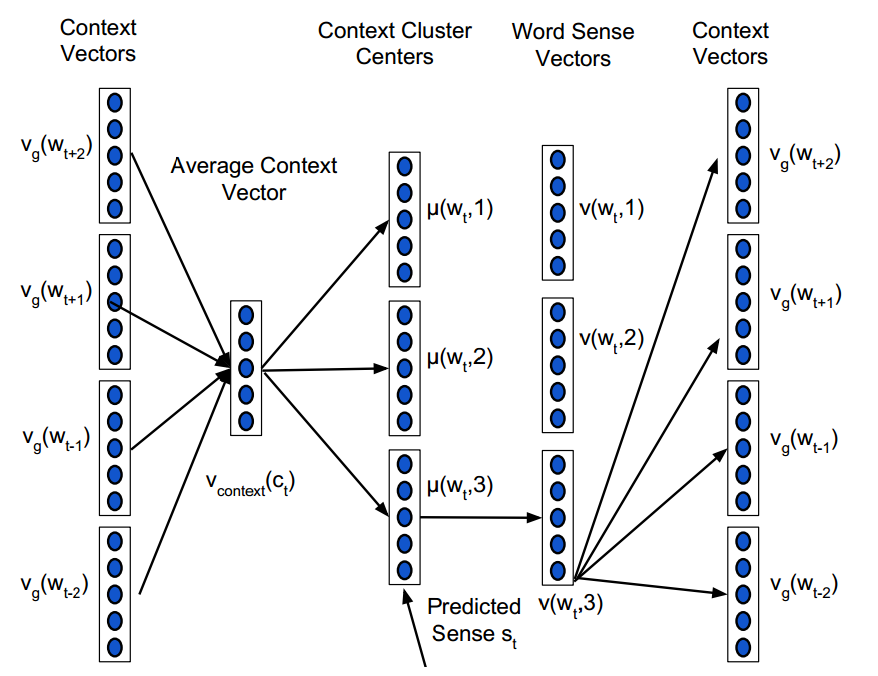
\includegraphics[width=0.9\textwidth]{MSSG} }
	\caption{Architecture of MSSG model with window size $R_t=2$ and $S=3$ }
	\label{fig:MSSG}
\end{figure} 

\paragraph{NP-MSSG}\ 

Unlike MSSG, in NP-MSSG model, the number of senses for each word is unknown and is learned during training. In the beginning, each word only has a global vector and does not have sense vectors and context clusters. When meeting a new context, for each word, the model will decide whether to create a new sense vector and a context cluster. When a word meets the first context, that is the first occurrence of this word in the corpus, the model creates the first sense vector and the first context cluster for this word.  After that, when there is a new context, the model will calculate all similarities between this word and current all context clusters, if the biggest similarity value is smaller than some given hyper-parameter $\lambda$, that is the new context is different from all current context clusters, the model will create a new context cluster and also a new sense vector as the beginning step. Otherwise, it will select the context with the biggest similarity value and do the same thing as what MSSG model do . Specifically, the selecting step can be described as the following formula :
$$s_t=\left\{
\begin{aligned}
&s(w_t)+1, &\mathrm{if}\  \max_{s=1,2,\ldots,s(w_t)}\{sim(\mu(w_t,s),v_{context}(c_t))\}<\lambda \\
&s_{max}, & otherwise \\
\end{aligned}
\right.
$$

where $s(w_t)$ is the number of senses (context clusters) of word $w_t$, $u(w_t,s)$ is the cluster center of $s^{th}$ cluster of word $w_t$ and $s_{max}=\arg\max_{s=1,2,…,s(w_t)}sim(\mu(w_t,s),v_{context}(c_t))$. 
